\documentclass[aspectratio=169]{beamer}

\usepackage[utf8x]{inputenx}
\usepackage{hyperref}
\usepackage[spanish]{babel}

\usetheme{Marburg}
%\usecolortheme{beaver}

\title[Modelos Cuant. de Redes Sociales]{Una Mirada General a los Modelos Cuantitativos de Redes Sociales}

\author[ggvy.cl]{George G. Vega Yon, Ph.D.}
\date{18 de Noviembre, 2021\\VII Reunión Latinoamericana de Análisis de Redes Sociales\\(Virtual)}
\institute[UofU Epi]{Division of Epidemiology\\University of Utah}

\begin{document}

\frame{\maketitle\vfill\hfill  \href{https://ggvy.cl}{\texttt{ggvy.cl}}}

\begin{frame}
	\frametitle{Contenidos}
\tableofcontents\pause
\vfill\hfill%
Descarga esta presentación desde \href{https://ggv.cl/slides/ars2021}{\color{blue}{\texttt{ggv.cl/slides/ars2021}}}
\end{frame}

\begin{frame}
	\frametitle{Motivación}
	``Tengo la pregunta ABC y los datos XYZ...\pause \bigskip
	\hfill\begin{minipage}{.8\linewidth}
		\raggedleft
		\Large ¿Qué \textbf{método} debo (puedo) utilizar\\\textbf{para lograr mi objetivo}?''
	\end{minipage}
\end{frame}

\section{Modelando Sistemas Complejos}

\frame{\title{Contenidos}\tableofcontents[currentsection]}

\begin{frame}
	\frametitle{Modelando Sistemas Complejos}
	Hoy por hoy
	\pause
	\begin{itemize}
		\item Estadística ``clásica'' asume que objeto de observación distribuyen de manera \textit{independiente} (\textit{siempre}) e \textit{idéntica}\pause{} (en general).\pause
		\item Entidades sociales no son independientes.\pause
		\item Asumir independencia puede ser problemático.\pause
		\item Programas y entrenamiento en el área apenas está comenzando.
	\end{itemize}\pause
	\vfill\hfill Sin embargo...
	\end{frame}

\begin{frame}
	\frametitle{Modelando Sistemas Complejos (cont. 1)}
	\begin{itemize}
		\item Contamos con mayor cantidad de datos.\pause
		\item Tenemos mayor poder computacional.\pause
		\item Existe una comunidad en ARS (SNA) que avanza desarrollo metodológico de manera acelerada.\pause
\end{itemize}

\vfill\hfill\large Es posible (e importante) crear una mirada sistemática del modelamiento de sistemas complejos.

\end{frame}

\begin{frame}
	\frametitle{Modelando Sistemas Complejos (cont. 2)}
	\begin{figure}
		\centering
		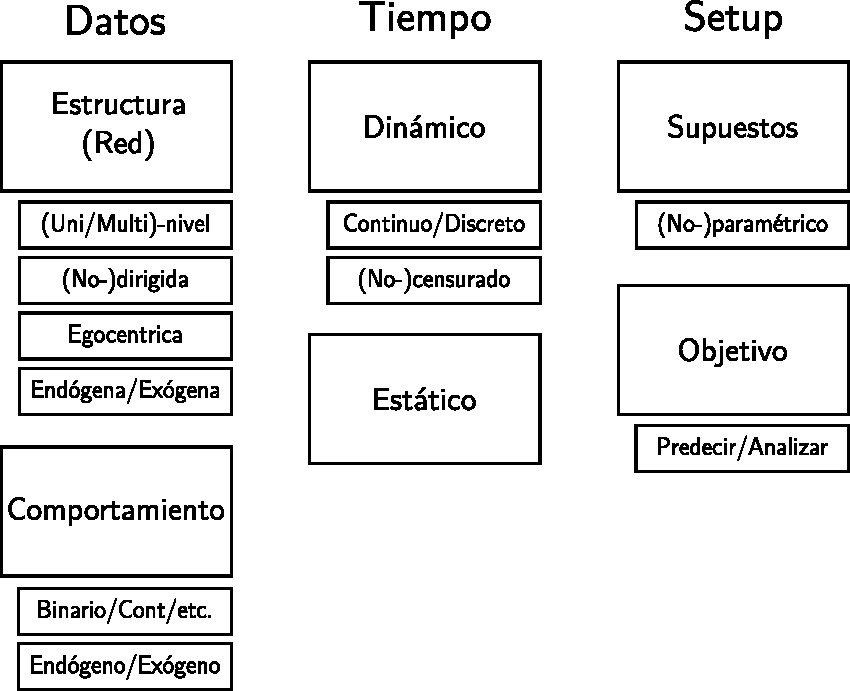
\includegraphics[width=.6\linewidth]{diagrama.pdf}
		\caption{Distintas dimensiones del análisis de redes sociales (perspectiva desde los datos.) Todas las entidades interactúan entre si.}
	\end{figure}

\end{frame}

\section{Propuesta de Clasificación}

\frame{\title{Contenidos}\tableofcontents[currentsection]}

\begin{frame}
	\frametitle{Propuesta de Clasificación}
	
	Dos dimensiones clave, \textbf{Estructura} vs \textbf{Comportamiento}, en particular\pause
	\begin{itemize}
		\item Estructura: Sólo nos interesa estudiar la red.\pause
		\item Comportamiento: Sólo nos interesa estudiar el comportamiento \textbf{en el contexto de la red} (fija).\pause
		\item Estructura x Comportamiento: Queremos ver como la red y el comportamiento interactúan entre si.
	\end{itemize}

\end{frame}

\subsection{Modelando Estructura}

\begin{frame}
	\frametitle{Clasificación: Estructura}
\pause
	\textbf{No paramétricos}
	\begin{itemize}
		\item \textbf{Network Bootstrap}: Errores estándar y comparación entre grafos
		\item \textbf{Network rewiring algorithms}: Identificación de \textit{motifs} condicionando en atributos observables (ej. secuencia o distribución de grado)
	\end{itemize}\pause	
	
	\textbf{Paramétricos}

	\begin{itemize}
		\item \textbf{Exponential Random Graph Models (ERGMs)} Incluyendo todas sus variantes, como por ejemplo, TERGMs, BERGMs, ERGMitos, etc.
		\item \textbf{Relational Event Models (REMs) y Dynamic Actor Network Models (DyNAMs)} Se observa una secuencia de interacciones en el tiempo.
	\end{itemize}
	
\end{frame}

\subsection{Modelando Comportamiento}

\begin{frame}
	\frametitle{Clasificación: Comportamiento}
\pause	
	\textbf{No paramétricos}
	\begin{itemize}
		\item \textbf{Test de permutación}: Simple o condicionado (ej. en \textit{in-degree})
	\end{itemize}
\pause
	\textbf{Paramétricos}
	\begin{itemize}
		\item \textbf{Test de autorrelación espacial}: Como la I de Moran.
		\item \textbf{Spatial Autoregressive Models}: Modelos lineales asumiendo errores autocorrelacionados con una estructura de red.
		\item \textbf{Regresiones rezagadas} Entidades actúan en base a exposición pasada.
	\end{itemize}
	
\end{frame}

\subsection{Modelando Estructura x Comportamiento}

\begin{frame}
	\frametitle{Clasificación: Estructura x Comportamiento}
\pause
	\textbf{No paramétrico}
	\begin{itemize}
		\item \textbf{Agent-Based Models (ABM)} Simulación de sistema complejo.
	\end{itemize}
\pause
	\textbf{Paramétrico}
	\begin{itemize}
		\item \textbf{Stochastic Actor Oriented Model (SAOM)} Proceso de Markov continuo donde individuos alteran su comportamiento/estructura condicionando en lo observado.
		\item \textbf{Discrete Exponential-Family Models (DEFMs)} Individuos toman acción sobre comportamiento y estructura de manera simultánea (en desarrollo...).
	\end{itemize}


\end{frame}

\section{Conclusiones}

\begin{frame}
	\frametitle{Conclusiones}
	\pause
	\begin{itemize}
		\item \textbf{Asumir independencia} no siempre es factible/útil, es más, todo lo contrario.\pause
		\item El \textbf{desarrollo} tecnológico y metodológico nos han \textbf{democratizado el análisis de sistemas complejos}.\pause
		\item Es importante crear un \textbf{marco teórico} para \textbf{guiar la práctica} del ARS (SNA).\pause
		\item Una primera propuesta: $\{\mbox{Estructura},\mbox{Comportamiento}\}$\pause
		\item Más en \url{https://gvegayon.github.io/appliedsnar}
	\end{itemize}
\end{frame}

\begin{frame}
	\centering
	\Huge ¡Gracias! \normalsize 
\titlepage%
\vfill\hfill  \href{https://ggvy.cl}{\texttt{ggvy.cl}}
\end{frame}

\end{document}